\chapter{Background}

\section{Fundamental Walking Dynamics and Control}
\subsection{Simple Models}
\subsubsection{Rimless wheel}
\subsubsection{Inverted Pendulum}
\subsubsection{Bipedal Spring Mass}

\subsection{Walking Controllers}
Shaping walking Dynamics through control

\subsubsection{Kinematic Centralized Controllers}

These approaches are usually model based and try to force the full system to
behave like a lower dimensional system. We can derive provably stable
controllers for lower order systems so if full order system behaves like lower
order system it will not fall.

\begin{itemize}
    \item ZMP preview control - forces robot to follow kinematics of lipm
    model
\end{itemize}

\subsubsection{Dynamic Centralized Controllers}
Force control allows robots to be compliant to external disturbances.

\begin{itemize}
    \item Model reduction approaches:        
        \begin{itemize}
            \item DRC  QP controllers force robots to follow dynamics of
                point mass systems
            \begin{itemize}
                \item Gaits are still statically stable
                \item dynamic in the sense that these controllers command forces
                    not kinematics
            \end{itemize}


            \item Spring mass model similar to previous approaches but force
            the robot to follow the dynamics of spring mass model

            \item Hybrid zero dynamics for full robots reduce dynamics to
            those of a single degree of freedom theo jansen walker
        \end{itemize}

    \item Heuristic Centralized/dynamic approaches
    \begin{itemize}
        \item Neural Network Dog controller - high level centralized neural
        network for commanding parameters of decentralized lower-level
        impedance controllers
    \end{itemize}
\end{itemize}

Centralized controllers rely heavily on models causes two problems
\begin{enumerate}
\item QPs and inverse dynamics result in unnatural, inefficient gaits to avoid
singularity which causes
\item Its unlikely we can model the diverse population of amputees in order
to derive centralized controllers that consider the joint amputee/prosthesis
dynamics.
\end{enumerate}
This motivates alternative heuristic decentralized controllers.

\subsubsection{Kinematic Decentralized Controllers}
    \begin{itemize}
        \item echo control
    \end{itemize}
\subsubsection{Dynamic Decentralized Controllers}
    \begin{itemize}
        \item raibert - motivation for landing leg angles
        \item virtual model control
        \item simbicon
        \item bioinspired controllers

        \item Applicable to prostheses
        \begin{itemize}
            \item not bio inspired
                \begin{itemize}
                    \item simbicon/impedance control
                    \item hybrid zero dynamics for prostheses
                \end{itemize}

            \item bio inspired

                We can derive another class of dynamic, decentralized
                controllers from biological models of animal and human
                locomotion. These models simulate locomotion at the level of the
                central nervous system, through simplified models of neural
                circuitry. 
                \begin{description}
                    \item[Central Pattern Generators (CPGs)]
                        
                    \item[neuromuscular model] 
                \end{description}
        \end{itemize}
   \end{itemize}

\section{Bioinspired Control for Prostheses}
\subsection{Impedance Control}

\subsection{Central Pattern Generators}
\subsubsection{Central Pattern Generators in Biology}
Central Pattern Generators (CPGs) are hypothesized nonlinear
oscillators, comprised of neurons in the central nervous system, that can
autonomously generate periodic neural activation
patterns~\citep{ijspeert2008central}.  \citet{brown1911intrinsic} first
suggested their existence based on experiments he conducted on decerebrated and
deafferented cats. In these experiments, \citeauthor{brown1911intrinsic} severed
both the afferent pathways (that carry sensory information) and efferent
pathways (that transmit higher level commands from the brain to motor neurons).
Despite the lack of high level control and sensory feedback, the cats still
displayed cyclical motions in their hind legs similar to those seen during
normal gait. This result suggests CPGs may play an important role in generating
locomotion controls in vertebrate animals. Similar cyclical neural activity
(called fictive locomotion) has been found in isolated lamprey spinal cords
\citep{cohen1980neuronal}, salamanders \citep{delvolve1999fictive}, and frog
embryos \citep{soffe1982tonic}. 

\begin{marginfigure}
    \centering
    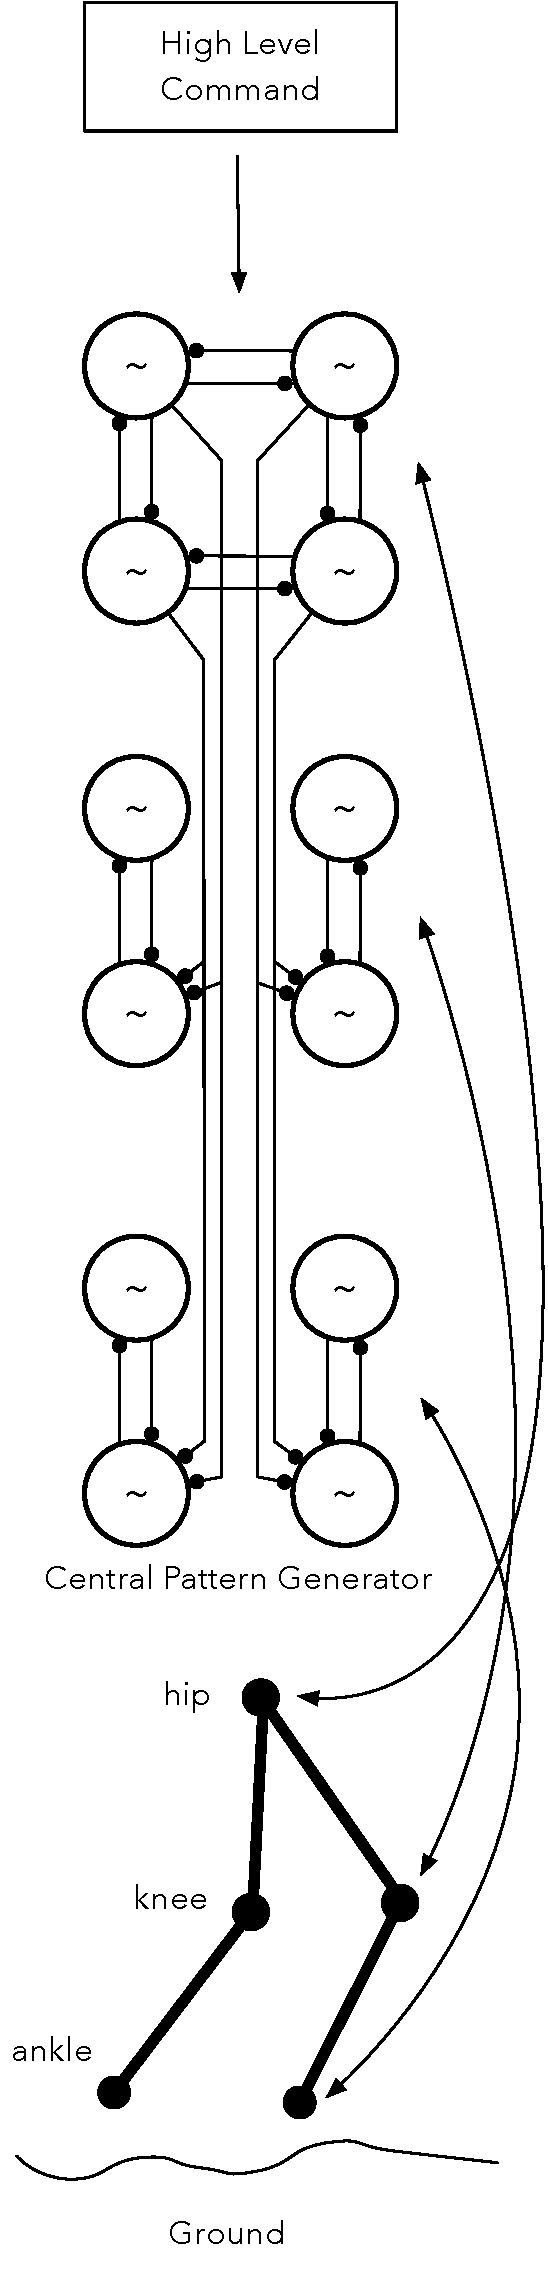
\includegraphics[height=6.25in]{CPG_diagram}
    \caption{Central Pattern Generator for bipedal locomotion as described in
    \citet{taga1991self}. Six neural oscillators receive feedback from and
    command joint torques for the hips, knees, and ankles of a planar biped
    model. A one dimensional high-level control signal enables control of speed
    and elicits gait transitions.}
    \label{fig:cpg_diagram}
\end{marginfigure}
Moreover, research has shown that stimulation of a region of the brain stem
called the Mesencephalic Locomotor Region (MLR) can manipulate the neural
activity generated by CPGs. For example, electrical stimulation of the MLR led
to gait transitions in both decerebrated cats \citep{shik1966control} and
salamanders \citep{cabelguen2003bimodal}.  Therefore, CPGs may serve as a form
of dimensionality reduction and decentralization for the biological control
system as low-dimensional, high-level signals from brain can shape the
high-dimensional, low-level CPG output. Consequently, CPGs may also represent
an attractive option for robotic legged locomotion controllers as
decentralization and dimensionality reduction are desirable properties in this
domain as well.

\subsubsection{Neuromechanical Models with CPGs}
The seminal work on CPG-based bipedal locomotion control is presented in
\citet{taga1991self}. In this model, a CPG neural network of six interconnected
oscillators describes the joint torques applied to a four link biped model.
Differential equations, first presented in \citet{matsuoka1987mechanisms} with
additional sensory feedback from joint and inertial link angles, describe the
output of the CPG network. The resulting biped model walks with a natural gait
featuring both single and double support and demonstrates robustness to a
variety of disturbances including changes to ground stiffness, damping, and
slope. Additionally, tuning a single parameter induced a transition from walking
to running in the model in a manner comparable to the biological gait
transitions observed after stimulation of the MLR.

CPGs have successfully controlled several bipedal humanoid robots. For example,
\citet{endo2005experimental} used \citeauthor{matsuoka1987mechanisms}'s
nonlinear oscillators along with by bio-inspired feedback pathways that regulate
ground reaction forces and body roll to generate desired foot trajectories for
the bipedal QRIO robot. As in \citeauthor{taga1991self}'s simulations walking
speed can be controlled via adjustment of a single parameter and the robot is
robust to changes in step height. Authors have also successfully employed other
nonlinear oscillator models. In \citet{shan2002neural}, a Recurrent Neural
Network generates oscillatory signals for a 20-DOF humanoid robot, HOAP-1, that
allow it to walk up and down stairs. In \citet{righetti2006programmable},
programmable ``Hopf'' oscillators \citep{righetti2006dynamic} learn desired
walking trajectories through entrainment enabling HOAP-2, a 25-DOF robot, to
walk forwards and backwards at varying speeds and step lengths.  

\subsubsection{CPGs for Prosthesis Control}
CPGs have also been proposed for controlling both mechanically-passive and
active lower limb prostheses.  \citet{nandi2009development} optimize CPG
parameters to fit recorded knee angle trajectories from healthy human subjects.
During walking, the CPG entrains desired knee motions to the oscillations of the
amputee's hip joint. The desired knee angles are achieved in a
mechanically-passive prosthesis via online adjustment of the knee damping.
Similarly, \citet{torrealba2010through, mora2012cybernetic} also use a CPG to
control a mechanically-passive variable damping prosthesis but use phase
resetting to synchronize the amputee and CPG dynamics. 

For active prostheses, \citet{geng2012design} suggest using a Hopf oscillators
to fit the trajectory of the knee angle during walking. \citet{guo2010study}
extend the idea of using a CPG for active prosthesis control by proposing a
hierarchical approach with a support vector machine (SVM) at the high-level
inferring amputee intent from EMG signals, and a CPG at the lower-level
determining the desired knee and ankle angles for an active transfemoral
prosthesis. However, in both cases, the authors do not provide experimental
results on real prosthesis hardware. Moreover, unlike in
\citeauthor{taga1991self}'s original work, these proposed CPG networks for
prostheses generate desired joint kinematics instead of torques. Consequently,
these controllers may not allow prostheses to exhibit the dynamism and
compliance we desire.

\subsection{Neuromuscular Reflexes}
\subsubsection{Neuromuscular Reflexes in biology}
Around the same time \citeauthor{brown1911intrinsic} hypothesized the existence
of central pattern generators, \citet{sherrington1910integrative,
sherrington1910flexion} suggested another mechanism for oscillatory neural
signals: chains of reflexes, or local feedback loops, that trigger in response
and entrain to sensory signals. \citeauthor{sherrington1910integrative}
identified complex, multi-joint, multi-limb reflex arcs involving both
excitation and inhibition in response to cutaneous stimulation in decerebrated
cats. Moreover, he observed rhythmic stepping behavior in decerebrated cats
suspended off the ground and concluded that the behavior emerged reflexively
based on proprioceptive signals emanating from the muscles themselves and not
from centrally generated oscillatory signals.

In animal experiments discussed earlier, while CPGs can go a long way towards
explaining locomotion neural activity, they still do not fully explain all
observed phenomena. Reflexes likely at least shape locomotion activation
patterns through entrainment, for example in Lamprey's movement of the tail
generates activation in the spinal chord of equal frequency
\citep{mcclellan1993mechanosensory} and phase resetting, as demonstrated by the
ability of decerebrated cats to walk on treadmills across a range of speeds
\citep{rossignol2000locomotion}.

For human and primate bipedal locomotion, the role of CPGs is more muddied and
the role of reflexes more evident than for decerebrated cats and simpler
vertebrate animals \citep{mackay2002central, vaughan2003theories,
nielsen2003we}. This is perhaps due to the demands of controlling the inherently
unstable dynamics of upright walking \citep{capaday2002special}. For example,
while rhythmic spinal activity has been observed in humans, it is not clear if
the neural signals are an example of autonomous fictive motion, indicative of a
CPG, or entrainment with stretch reflexes in leg muscles
\citep{capaday2002special, stewart1991modulation}. In this case, we can also
look to robotics to provide insight about biology: in the previously discussed
experiments on humanoid robots controlled by CPGs, a significant reduction in
robustness was observed after blocking sensory feedback pathways
\citep{endo2005experimental, righetti2006programmable} indicating CPGs alone may
not fully explain bipedal locomotion. Whereas research has not yet clearly
established the presence of a CPG driving human locomotion, research has
identified many reflexes that contribute to locomotion such as the Hoffman
reflex (H-reflex) of the soleus ankle plantarflexor muscle
\citep{capaday1987difference}, stretch reflex in the soleus
\citep{yang1991contribution}, soleus force feedback \citep{grey2007positive},
and cutaneous reflexes that induce withdrawal responses \citep{yang1990phase}. 

\subsubsection{Neuromuscular Models with Reflexes}
\begin{marginfigure}
    \centering
    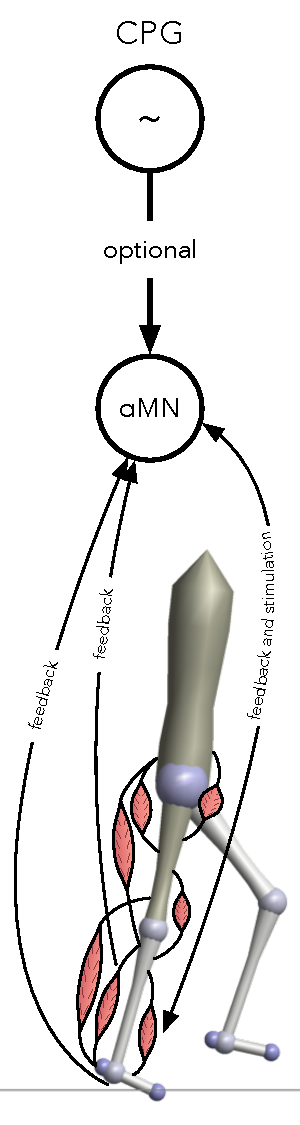
\includegraphics[height=5.5in]{reflex_diagram} 
    \caption{Neuromuscular models with reflex feedbacks. The model developed by
    \citet{ogihara2001generation} activates individual muscles according to the
    activity of a CPG and proprioceptive reflexes that can involve the muscle
    itself, other muscles, and ground contact sensing.  \citet{geyer2010muscle}
    does away with the CPG and achieves locomotion with only reflex feedbacks.}
    \label{fig:reflex_diagram}
\end{marginfigure}
To model the potential interplay between muscular reflexes and CPGs in human
locomotion \citet{ogihara2001generation} extend the model presented in
\citet{taga1991self} by adding muscles stimulated by alpha motor neurons. This
model simulates nine muscles of the leg, each stimulated by an alpha motor
neuron that receives input from a CPG oscillator and proprioceptive feedback
from one or more muscles. The muscles produce forces according to their state
and activation input (computed using models presented in
\citet{pierrynowski1985physiological} and \citet{davy1987dynamic}). These forces
are applied to constant moment arms in order to produce joint torques summed
about joints. The authors optimize the cost of transport of transport of them
model with a genetic algorithm and achieve a gait with human-like kinematics,
kinetics. Moreover, the forces produced by many of the muscles resemble those
produce during human locomotion. Despite the fact that the CPG used in this
model received no feedback signals, the resultant gait still exhibited a small
degree of robustness to perturbations although not as much as
\citeauthor{taga1991self}'s model. The author's attribute the robustness to the
stabilizing feedback provided by muscle reflexes. 

Whereas models and robot experiments show reflexes are vital for maintaining
bipedal gait stability, the same cannot be said about CPGs. In fact, as shown by
\citet{geyer2010muscle}, it is possible to simulate robust and human-like
bipedal locomotion using only reflexes. This work, employs a neuromuscular
model, similar to that used in \citet{ogihara2001generation}, but does away with
the feed forward CPG stimulations sent to alpha motor neurons. Instead,
\citeauthor{geyer2010muscle} hypothesize the existence of several force and
length muscle reflexes that seek to implement three key aspects of bipedal
locomotion: compliant leg behavior, preventing joint over extension, and trunk
stabilization. The gait achieved by this model is more robust and more
accurately reproduces kinematics, kinetics, and ground reaction forces seen in
human walking than \citeauthor{ogihara2001generation}'s model and produces
human-like stimulations for many of its muscles.

While we cannot say based on this result alone that CPGs do not play an
important role in human locomotion, the fact that human locomotion can emerge
from purely reflexive controls increases the attractiveness of using this
approach for prosthesis control. This is because the reflex-only paradigm may be
easier to design and optimize than the CPG+reflex paradigm for two reasons:
First, the reflex connection graph used by \citet{geyer2010muscle}'s reflex-only
model is much more sparse than that used by \citet{ogihara2001generation}
CPG+reflex model. Using a sparse set of reflexes and no CPG reduces the number of
parameters that we must tune in order to achieve locomotion. Second, the
reflexes in the reflex-only model are functionally motivated, which may increase
our intuition about the role of each reflex and assist our ability to tune the
model's parameters. This is evidenced by the fact that
\citeauthor{geyer2010muscle} hand tuned the parameters of their model whereas
\citeauthor{ogihara2001generation} used a genetic algorithm.  Moreover,
functionally motivated feedbacks used in the reflex-only approach has allowed
further research to extend this model to include swing leg placement
\citep{desai2013muscle}, 3D locomotion, running, speed changes, stair and slope
negotiation, turning, and obstacle avoidance \citep{song2015neural}.  

The robustness properties exhibited by neuromuscular control are especially
relevant to our goal of developing a robust prosthesis control that will help
transfemoral amputees avoid falls. In \citet{song2015neural} the author's
improve the model's robustness by incorporating reflexes that place the swing leg
into target landing angles. The authors optimize this model to achieve a
combination of robustness and energy efficiency.  The resulting gait can walk on
terrains featuring random steps up to $\unit[\pm 6]{cm}$ (50 \% success rate)
and reject pushes in both the forward and backward directions at various points
in the gait cycle. In another work, \citet{murai2011neuromuscular} subject a
neuromuscular model, initially trained to match kinematic data of single
subject, to impacts during early and late swing. They find the learned model
exhibits elevating and lowering strategies despite not being explicitly trained
to do so.

\subsubsection{Neuromuscular Reflexes for Prosthesis Control}
\begin{marginfigure}
    \centering
    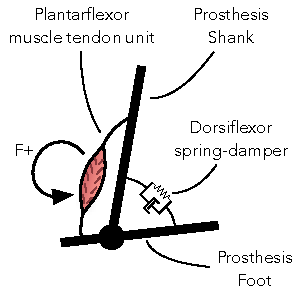
\includegraphics[width=\linewidth]{eilenberg_diagram} \caption{Neuromuscular
    model used by \citet{eilenberg2010control} to control an active ankle
    prosthesis. During stance, a virtual muscle driven by positive force
    feedback, generates plantarflexion torque. During swing, a virtual spring
    damper provides dorsiflexion torque to prevent toe scuffing.}
    \label{fig:eilenberg_diagram}
\end{marginfigure}
Motivated by the robustness and natural gait achievable by neuromuscular
reflex control, past research has applied this model to active prostheses and
exoskeletons. \citet{eilenberg2010control} applied a simplified version of the
control to a powered ankle prosthesis (\cref{fig:eilenberg_diagram}). In this
work, the neuromuscular model was reduced to a single ankle plantarflexor muscle
driven by a positive force feedback reflex during stance. During swing, the
control applies torque to dorsiflex the ankle according to a virtual spring
damper model. In amputee testing of a prosthesis controlled by the neuromuscular
model the control produced ankle kinematics and kinetics similar to those
observed in healthy human walking. Significantly,
\citeauthor{eilenberg2010control} found evidence that the robustness and
entrainment properties observed in neuromuscular model simulations may carry
over to amputee gait as well. The author's note that the prosthesis
automatically adapts torque output when walking on slopes, producing more
plantarflexion torque when walking up slopes and less when walking down slopes.
Additionally, \citet{markowitz2011speed} found that a similar neuromuscular
reflex model automatically produced more ankle plantarflexion work as the
amputee increased his gait speed.

\subsubsection{EMG-based Control}\label{sec:emg_control}

The inclusion of user intent recognition via surface electromyography (EMG)
signals represents an interesting extension of neuromuscular reflex prosthesis
control. In these approaches, muscle activity in the residual limb is directly
measured via EMG sensors embedded in the amputee's prosthesis socket. These EMG
sensors are then used to control the torque generation of the amputees leg
prosthesis. Because neuromuscular models describe how joint torque is generated
in response to muscle activations, a natural approach is to use the EMG signal
in reflex pathways in order to activate virtual muscles. This is the approach
proposed by \citet{wu2011electromyography}. In this work,
\citeauthor{wu2011electromyography} control an active transfemoral prosthesis
using EMG sensor readings from the residual thigh to activate virtual knee
flexor and extensor muscles according to a linearised Hill muscle model. The
resulting prosthesis control allowed an intact subject wearing the prosthesis
via an able-bodied emulator to achieve nearly normal gait. In a similar
approach, \citet{wang2013proportional} use EMG signals to modify the gain on a
positive torque feedback loop (similar to positive force feedback used in
\citet{geyer2010muscle}) in order to control ankle plantarflexion torque. As
seen in healthy human walking, toe off angle and ankle net work increased with
increasing walking speed.

These two works have demonstrated that neuromuscular approaches have enabled EMG
based control to go beyond its typical application of high-level mode
recognition. For example, \citet{huang2009strategy, huang2011continuous}, and
\citet{hargrove2015intuitive} recognize walking modes, such as level ground
walking, ramp and stair ascent, and ramp and stair descent, by training
classifiers on features of EMG and mechanical sensor data. In contrast, the EMG
+ neuromuscular approaches allow to use typically noisy EMG sensor data for
low-level continuous control. \citet{wu2011electromyography} and
\citet{wang2013proportional} propose that because EMG + neuromuscular approaches
model physiologically plausible feedback loops and dynamics, they may allow
amputees to use muscle activations to control their prostheses in an intuitive
way.

\subsection{Conclusion} 
In summary, simulations and implementations of the neuromuscular reflex control
approach have repeatedly demonstrated its ability to generalize to a variety of
situations and exhibit robustness to a variety of disturbances. Due to the gait
deficits and fall risk transfemoral amputees face, these two properties make
this control paradigm very attractive for application to transfemoral prostheses
. Moreover, neuromuscular approaches have been successfully extended with EMG
sensor feedback from amputees' residual limbs, enabling intuitive low-level
prosthesis control. In contrast, other control approaches for prostheses such as
impedance control have not demonstrated these properties. Importantly,
neuromuscular control addresses challenges 1 and 2 of amputee
locomotion~(\cref{sec:challenges}) as we can implement them via a decentralized,
sparse set of reflexes and they allow for dynamism by providing joint torque
commands via muscle models.

As yet, there have not been any published works applying neuromuscular reflex
control to active knee and ankle transfemoral prostheses. Therefore, in this
thesis, we work towards this goal with the hope of improving transfemoral
amputee gait robustness and naturalness. \Cref{sec:neuro_model} will review the
details of the particular neuromuscular implementation used in this thesis.

\section{Prosthesis Design}\label{sec:pros_design}

We can trace efforts to build an active knee-ankle prostheses to the seventies
when \citet{flowers1974use} created an active knee-ankle prosthesis emulator in
order simulate potential control schemes. This prosthesis used a hydraulic
actuator capable of producing $\unit[90]{N \cdot m}$ of torque and
$\unitfrac[0.5]{rev}{s}$ of no-load speed, sufficient for simulation of passive
prostheses. With this device, \citet{donath1974proportional} tested proportional
EMG control, a problem researchers are still investigating today
(see~\cref{sec:emg_control}). Indeed, this line of research proved to be far
ahead of its time, as most relevant research in active lower-limb prostheses
design has occurred only in the last ten years. The recent interest in active
knee ankle prostheses has been spurred by hardware improvements that allow
designs to approach the strength, speed, and low weight of the biological leg.
Enabling technologies include power-dense brushless motors, motor controllers,
and lithium-ion batteries, inexpensive microcontrollers and inertial measurement
units (IMUs), and strong but light composite materials such as carbon fiber.
With these advancements, engineers have successfully designed prostheses to meet
or exceed the requirements for walking~(\cref{tab:walking_requirements}).
\begin{margintable}
  \centering
  \begin{tabular}{lll}
    \toprule
    & Ankle Max & Knee Max \\
    \midrule
    Velocity & \unitfrac[0.72]{rev}{s} & \unitfrac[1.17]{rev}{s}\\
    Torque & $\unit[130]{N \cdot m}$ & $\unit[57]{N \cdot m}$\\
    Power & \unit[350]{W} & \unit[120]{W}\\
    \bottomrule
  \end{tabular}
  \caption{Required knee and ankle torque, velocity, and power for walking
  (\unitfrac[1.40]{m}{s} average speed, scaled to \unit[85]{kg} subject,
  data from \citet{winter2009biomechanics})}
  \label{tab:walking_requirements}
\end{margintable}

In this \namecref{sec:pros_design}, we review a number of recent prosthesis
designs and analyze their ability to enable dynamic locomotion
(\hyperref[sec:challenges]{challenge 1} of transfemoral prosthesis locomotion).
To address this challenge, prostheses should be able to regulate their output
joint torques and behave as though they have inertial properties similar to
that of a normal human leg. This will ensure that the prosthesis will emulate
the energy efficient gaits of normal walking and remain compliant to unforeseen
disturbances and uneven terrain.

\subsection{Direct Drive Transfemoral Prostheses}\label{sec:direct_drive}

The most common approach for active transfemoral prosthesis design employs
electric motors, coupled to transmissions, that directly drive the knee and
ankle joints. The transmissions may utilize a combination of gears, chains,
belts, ball screws, and four-bar-mechanisms in order to increase the torque
output of the actuator, at the expense of speed, in order to satisfy the
requirements listed in \cref{tab:walking_requirements}. A successful line of
transfemoral prostheses following this design paradigm comes from Vanderbilt
university. The first prosthesis in this line \cref{fig:vanderbilt_prostheses}a
used a pair of ball screw transmissions and brushless motors capable of
\unit[200]{W} of continuous power output to drive its knee and ankle joints
\citep{sup2009preliminary}. 

With these actuators, the knee motor can achieve the required peak torque and
peak power intermittently (\cref{tab:walking_requirements}). However, the ankle
motor may be overly stressed due to the high requirements of walking. To remedy
this, this prosthesis includes of a unidirectional parallel spring in the ankle
that reduces the required ankle motor torque. As shown in figure
\cref{fig:ankle_torque_vs_angle}, during level ground walking, a linear torsion
spring can account for a significant portion of the ankle's torque versus angle
relationship. Therefore, incorporating a spring into the ankle offloads this
portion of the torque from the motor. The ankle motor only needs to provide the
delta between the desired output torque and the linear spring. As a result, the
spring reduces motor energy consumption, heat generation, and transmission wear.

\begin{marginfigure}
    \centering
    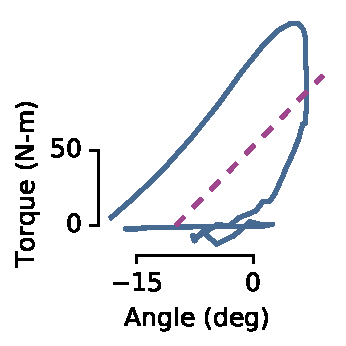
\includegraphics[width=\linewidth]{ankle_torque_vs_angle}
    \caption{Torque vs angle relationship for the ankle during level ground
    walking (blue solid). A linear spring relationship captures a significant
    portion of ankle function (purple dashed). Data from
    \citet{winter2009biomechanics} scaled to 85 kg subject.}
    \label{fig:ankle_torque_vs_angle}
\end{marginfigure}

Further improvements resulted in two more generations of prostheses
(\cref{fig:vanderbilt_prostheses}b \& c) \citep{lawson2013control,
lawson2014robotic}. These versions replaced the ball screw transmissions with
multi-stage belt/chain due to the improved packaging and reduced noise and wear
they afford (Michael Goldfarb, personal communication, September 18, 2013). With
these prostheses, researchers have extensively tested a variety of control
strategies including impedance control \citep{sup2009preliminary,
sup2011upslope, lawson2013control, lawson2014robotic}, EMG-based control
\citep{ha2011volitional, varol2010multiclass}, minimum jerk trajectory following
\citep{lenzi2014minimum}, and virtual constraint control
\citep{gregg2014virtual}. 

\begin{figure*}[t]
    \centering
	\begin{subfigure}[t]{0.3\textwidth}
    	\centering
        %\includegraphics{}
        \missingfigure{Gen 1}
        \caption{Generation 1 used ball screw transmissions, \unit[200]{W}
        brushless motors, and a unidirectional parallel spring in the ankle that
        reduced motor torque requirements \citep{sup2009preliminary}.}
        \label{fig:vanderbilt_gen_1}
	\end{subfigure}
	\begin{subfigure}[t]{0.3\textwidth}
    	\centering
        %\includegraphics{}
        \missingfigure{Gen 2}
        \caption{Generation 2 replaced ball screws with custom gear-based
        transmission that is less noisy and durable \citep{lawson2013control}.}
	\end{subfigure}
	\begin{subfigure}[t]{0.3\textwidth}
    	\centering
        %\includegraphics{}
        \missingfigure{Gen 3}
        \caption{Generation 3 features a modular design with separable knee and
        ankle units \citep{lawson2014robotic}.}
	\end{subfigure}
    \caption{Vanderbilt University's Robotic Transfemoral Prostheses.}
    \label{fig:vanderbilt_prostheses}
\end{figure*}

Additional prostheses in the direct drive category include AMPRO
\citep{zhao2016first}, and commercially available active knee and ankle
prostheses: the Össur Power Knee and Proprio Foot. The AMPRO prosthesis features
two 374 W motors coupled to Harmonic Drive transmissions.
\citet{zhao2016first}, use this prosthesis to asses the merits of virtual
constraint. The Össur Power Knee features an electric motor that can provide
torque to facilitate sit-to-stand motions, stair climbing, and active extension
and flexion during walking. The Proprio Foot also features electric actuation
that allows it to adapt to terrain and dorsiflex the ankle during swing to help
avoid trips. 

\subsubsection{Torque Control Strategies for Direct Drive
Prostheses}In order to achieve dynamic locomotion capabilities, it is crucial that
prosthesis designs allow for closed loop control of torques. To do this control
system must be able to accurately measure the torque at the joint output. There
are two main strategies for torque measurement used by direct drive prostheses.

The first strategy is to measure the current draw of the motors windings, which
is related linearly to the motor torque. One can then multiply this measurement
by the gear ratio to obtain an estimate of the output joint torque. This is the
method used by Generations 2 and 3 of the Vanderbilt prosthesis as well as the
AMPRO prosthesis. The benefit of this method is that it utilizes existing
hardware and allows one to use high frequency current control modes of motor
drivers. However, a drawback of this method is that it measures the torque
before the transmission. Consequently, it does not account for frictional
losses, which can be difficult to model, especially for geared systems. A
strategy that deals with this problem is to install load cells in series with
the motor after the transmission, as was done on Generation 1 of the Vanderbilt
prosthesis. With this method, the closed-loop control can compensate for
frictional losses as they are included in the torque measurement. 

However, this method may still not address a second problem sluggish passive
dynamics caused by reflected inertia and damping. Reflected inertia refers to
the apparent magnification of motor rotor and gearing inertia on the outside of
gearbox.  We can derive this effect through Newton's second law for the geared
motor
\begin{align}
    J_i \ddot{\theta}_i = \tau_i - b_i \dot{\theta}_i.
\end{align}
Here, $\theta$ and its derivatives refer to angular states of the motor, $b$
is the damping constant, $J$ is the inertia and $\tau$ is the motor torque. We
use subscript $i$ to refer to these quantities as seen before the gear
reduction, and subscript $o$ to refer to those quantities reflected outside of
the motor. Plugging in $\theta_i = n \theta_o$ and $\tau_i = \frac{1}{n}
\tau_o$, where $n$ is the gear ratio, and multiplying through by $n$ yields
\begin{align}
    J_i n^2 \ddot{\theta}_o &= \tau_o - b_i n^2 \dot{\theta}_o \\
    \implies \quad J_o \ddot{\theta}_o &= \tau_o - b_o \dot{\theta}_o.
\end{align}
These equations show that the inertia and damping of the motor rotor get
amplified by the square of the gear ratio. As prostheses may often use gear
ratios in excess of 100:1, this effect can be substantial. 

\begin{table}
  \centering
  \begin{tabular}{lll}
    \toprule
    & Knee & Ankle \\
    \midrule
    rotor inertia & $\unit[0.035]{kg \cdot cm^2}$ 
        & $\unit[1.210]{kg \cdot cm^2}$\\
    gear ratio & 176:1 & 115:1 \\
    reflected inertia & $\unit[0.11]{kg \cdot m^2}$ & 
        $\unit[1.6]{kg \cdot m^2}$\\
    human inertia & $\unit[0.66]{kg \cdot m^2}$  & $\unit[0.019]{kg \cdot m^2}$\\
    percent increase & 17\% & 8400\% \\
    \bottomrule
  \end{tabular}
  \caption{Estimated reflected inertia at knee and ankle joints of Generation 3
  Vanderbilt Prosthesis \citep{lawson2014robotic}. Motor data taken from Maxon
  Motors Catalog\citep{maxon_flat_motor,
  maxon_ec4pole} Knee reflected inertia compared to inertia of human shank and
  foot about knee. Ankle inertia compared to human foot about its center of
  mass. Human inertias estimated from \citet{winter2009biomechanics} for a
  \unit[85]{kg}, \unit[1.7]{m} tall person.}
  \label{tab:vanderbilt_reflec_interita}
\end{table}

For example, \cref{tab:vanderbilt_reflec_interita} shows the calculated
reflected inertias of the Maxon Motors used in Generation 3 of the Vanderbilt
prosthesis and compares the values to the estimated inertia of the shank and
foot about the knee and the foot about its center of mass. We see that at the
knee, the reflected inertia is roughly 17\% of that of the human shank and foot.
In practice, this value is likely several times higher after including the
inertia of the encoder, bearings, and gearing. Consequently, we can estimate
that the reflected inertia may be on the order of the leg itself. At the ankle,
the reflected inertia of the rotor alone is several orders of magnitude more
than that of the foot and more than twice that of the shank and foot. When we
also consider reflected damping and friction, the dynamics of prosthesis system
may be significantly slower than assumed.

The increase in joint impedance that transmissions create could present an issue
when attempting to execute dynamic behaviors involving impact such as running or
trip recovery. In an impact event, the impulse will move through the system at
the speed of sound through metal, roughly \unitfrac[6420]{m}{s} for aluminum
\citep{lide2004crc}. If the prosthesis is \unit[0.5]{m} long, the shock will
traverse its length in \unit[0.00008]{seconds}. This is about 10 times faster
than the typical 1000 Hz control frequency of prosthesis control systems,
rendering closed loop torque control with load cells unresponsive. Consequently,
the impact could cause damage to gearing and discomfort for the amputee.

%Reflected Inertia
%Vanderbilt gen 3 ankle = 1210 g*cm^2 * 115^2 in kg*m^2 = 1.6 kg*m^2
%Vanderbilt gen 3 knee = 35 g*cm^2 * 176^2 in kg*m^2 = 0.11 kg*m^2

%human leg for 1.7 85 kg = 0.6575 kg*m^2
%human foot for 1.7m 85 kg = 0.0187 kg*m^2

\subsection{Design of Dynamic Prostheses}

In contrast to the direct drive actuation discussed in the previous subsection,
prostheses that employ series elastic actuation may be better poised to achieve
dynamic locomotion \citep{pratt1995series}. This actuation scheme (illustrated
in \cref{fig:sea_diagram}) aims to solve the torque measurement and impedance
amplification caused by transmissions by placing a spring in series with the
actuator. Measuring the deflection of the spring allows for accurate closed-loop
control of the joint torque. Moreover, the spring low-pass filters external
impulses, granting the control system more time to move the motor rotor in
response to the external load. In addition to finding use in prostheses, series
elastic actuators have been employed on a number of bipedal robots that seek to
achieve dynamic locomotion such as M2V2 \citep{pratt2008design} and ATRIAS
\citep{grimes2013atrias}.

\begin{marginfigure}
    \centering
    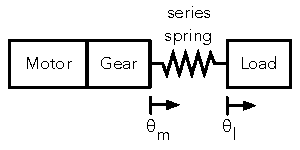
\includegraphics[height=6.25in]{sea_diagram}
    \caption{Series elastic actuation inserts a spring between the gear output
    and the load (here drawn as linear actuator for simplicity). Torque is
    measured via the spring deflection, $\tau = k(\theta_l - \theta_m -
    \theta_0)$ where $\tau$ is the output joint torque, $k$ is the spring
    constant, and $\theta_l$ and $\theta_m$ are the load and motor positions and
    $\theta_0$ is the spring's rest length.}
    \label{fig:sea_diagram}
\end{marginfigure}

Series elastic actuators have found use in a variety of transtibial and
transfemoral prostheses. We can further split these applications into two
categories, those that optimize the spring stiffness for control bandwidth
subject to shock tolerance, and those that optimize spring stiffness to optimize
efficiency.

\subsubsection{Springs for Bandwidth and Shock Tolerance}

Adding a spring between the gear and load introduces additional dynamics between
external torques and torques applied to the gearbox as external torques must
physically displace the load before the generate torque on the motor. This
property can improve the shock tolerance of SEA actuators over that of direct
drive motors~\citep{robinson2000design}. However, by the same token, the SEA
also introduces additional dynamics between motor torque and load torque, hence
reducing force control bandwidth. Therefore, a trade-off exists between the
compliance of the actuator and speed with which it can generate desired torques.

\citet{au2007biomechanical, au2008powered} design a powered ankle prosthesis
with this trade off in mind. In this work, the authors find that 

\begin{description}
    \item[Biom lineage]
        series springs for shock tolerance parallel spring for bandwidth] powered ankle
        prostheses with series elastic spring for shock tolerance and parallel spring
        for large force bandwidth improvement. Eventually developed into biom ankle
        prosthesis \citep{au2007biomechanical, au2008powered}.
    \item[Prosthesis emulators]
\end{description}

\subsubsection{Springs for energy efficiency}
\begin{description}
\item[Sparky series] use series springs for energy
efficiency\citep{hitt2007sparky} later version added inversion
eversion\citep{bellman2008sparky}.
\item[MIT transfemoral prostheses] 
    \begin{description}
        \item[Agonist-Antagonist Active Knee Prosthesis] allows for simultaneous
        adjustment of joint position and stiffness \citep{martinez2008design}
        \item[CSEA] knee spring to capture conservative torque
        \citep{rouse2014clutchable} 
    \end{description}
\end{description}

We take inspiration from Biom, Atrias, Emulators  

\section{Balance Recovery for Prostheses}
